\documentclass{article}
\usepackage[utf8]{inputenc}
\usepackage{amsmath}
\usepackage{float}
\usepackage{graphicx}
\usepackage{float}
\usepackage[a4paper,top=2cm,bottom=2cm,left=2cm,right=2cm,marginparwidth=2cm]{geometry}

\title{Pre-Informe Trabajo final}
\author{Grupo 2}
\date{Mayo 2020 - DSP}

\begin{document}
\maketitle
\section{Marco teórico}
Con la finalidad de explicar el funcionamineto de la transformada de Wavelet se comenzara respondiendo la siguiente pregunta:
¿Porqué es importa la transformada Wavelet en el procesamiento digital de señales?.\\
Para responder esta pregunta primero definimos que es una señal estacionaria y una señal no estacionaria:
\begin{itemize}
    \item Señal estacionaria: en este tipo de señales la frecuencia no varia en el tiempo (Fig 1).
    \begin{figure}[H]
        \centering
        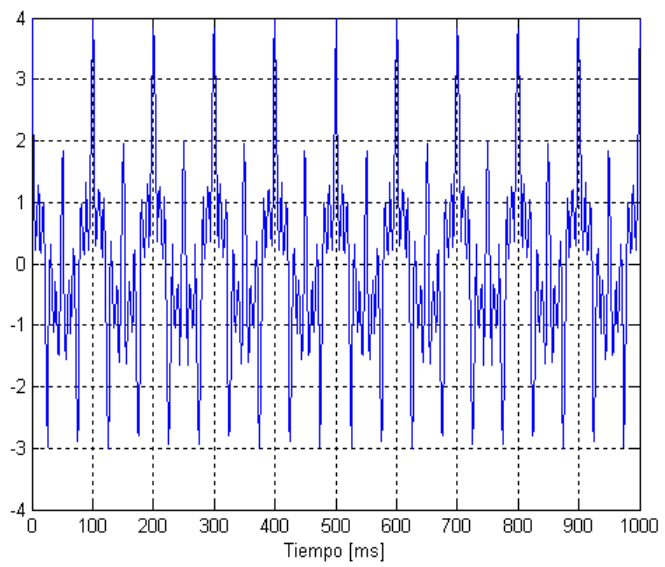
\includegraphics[scale=0.45]{Fig/1}
        \caption{Ejemplo de señal estacionaria. Fuente:}
        \label{fig1}
      \end{figure}
    \item Señal no estacionaria: este tipo de señales presenta variaciones en las componentes de frecuencia a lo largo del tiempo (Fig 2).
    \begin{figure}[H]
        \centering
        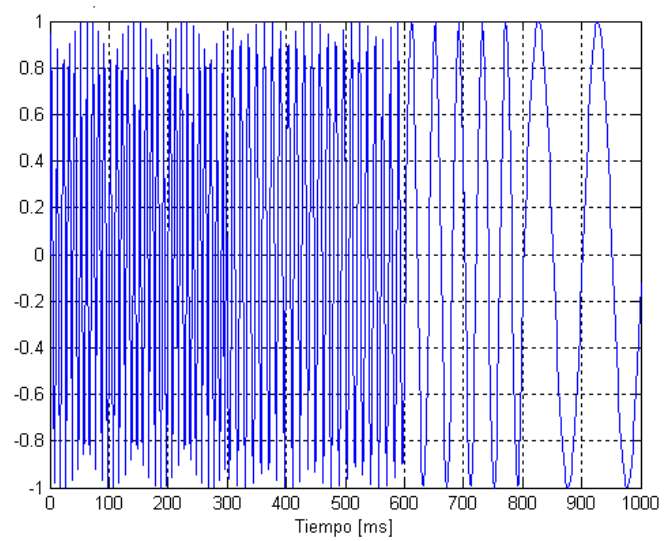
\includegraphics[scale=0.45]{Fig/2}
        \caption{Ejemplo de señal no estacionaria. Fuente:}
        \label{fig1}
      \end{figure}
\end{itemize}
Si queremos extraer información de este tipo de señales es inmediato pensar en el analisis en frecuencia y por lo tanto en la transformada de Fourier:
\begin{equation}
    X(\Omega) = \int_{-\infty}^{\infty} x(t)e^{-j\Omega t}dt
\end{equation}
Esta ecuación brinda una representación en el dominio de la frecuencia de una señal estacionaria, ya que $\Omega$ esta definida para todo el 
intervalo $(-\infty,\infty)$. Por lo tanto, la transformada de fourier brinda resultados óptimos cuando el contenido de frecuencia de la señal no cambia en el tiempo. Si se requiere 
analizar una señal como, por ejemplo, la de la figura 2 con la transformda de fourier, obtendriamos las componentes de frecuencia presentes en esta señal pero no tendriamos ningun tipo de 
iformacíon temporal del momento en el que cambia la frecuencia y tampoco donde se produce el spike \footnote{Irregularidad en la señal VER}. Esta información es muy importante para analizar, por ejemplo, sistemas físicos donde se quiera averiguar el tiempo en que la frecuencia de oscilación o la densidad de un material x cambie,
y utilizarla para encontrar el fenómeno que la produce.\\
AGREGAR FIGURAS QUE MUESTREN LO ANTERIOR Y TAMBIEN LO DEL SPIKE\\

La Transformada Wavelet o tambien llamada Transformada ondeleta, soluciona los problemas que presenta la 
transformada de Fourier con señales no estacionarias. Utilizando un análisis multiresolución con ventanas de longitud variable las cuales se adaptan a la frecuencia de la señal.
Las ventanas utilizadas por la Transformada de Wavelet cumplen lo siguiente:
\begin{itemize}
    \item Si se necesia mayor precisión en baja frecuencia la ventana tiene un intervalo temporal grande.
    \item Si se necesita mayor información en alta frecuencia, la ventana tendra un intervalo temporal mas pequeño.
\end{itemize}
\begin{figure}[H]
    \centering
    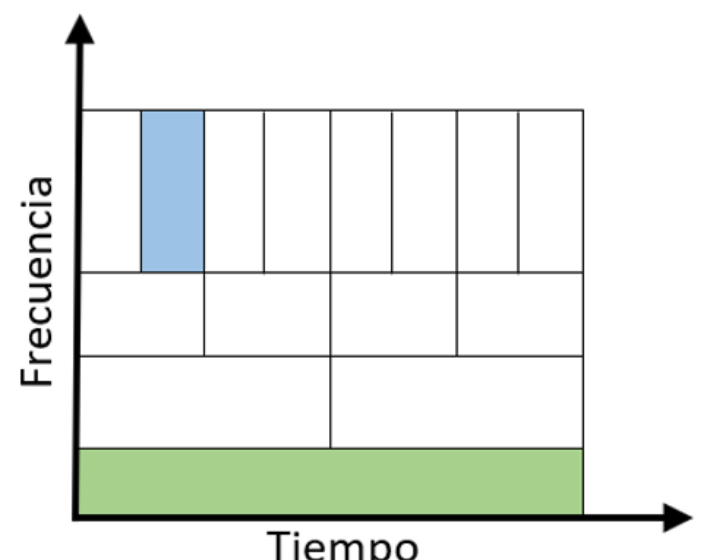
\includegraphics[scale=0.35]{Fig/66}
    \caption{Esquema de las ventanas en la transformada Wavelet}
    \label{comp}
\end{figure}
En la figura \ref{comp} se observa en color verde la ventana que cumple el primer item. Es decir, se requiere analizar componentes de baja frecuencia y por lo tanto el intervalo temporal es grande (ventana amplia). El otro item se ve en la ventana azul, para un analisis 
en grandes frecuencias la ventana temporal sera pequeña (ventana angosta).
Estas ventanas presentadas de forma esquemática en la figura \ref{comp} tiene una forma especifica y es lo le da el nombre a esta transformada. Una \textit{Wavelet} es una ``pequeña onda'' que tiene su energia concentrada en un periodo de tiempo determinado, son de duración definida, irregulares y asimétricas, lo que les permite 
adaptarse y converger de mejor manera a la señal que se quiere analizar. Haciendo un paralelismo con la tranformada de fourier donde se utilizan senos y cosenos para representar una señal, aqui se utiliza una \textit{Wavelet Madre} y sus ``Wavelets hijas'' o ``átomos de wavelet''. Es decir, mientras que con fourier se agregan senos y cosenos para lograr 
una mejor representación, aqui se agregan Wavelets hijas. Con el fin de explicar esto planteamos la familia wavelet (o wavelets hijas):
\begin{equation}
    \label{WM}
    \psi(a,b)(t)= \frac{1}{\sqrt{a}} \psi(\frac{t-b}{a})
\end{equation}
Las wavelets hijas mencionadas corresponden a una traslación y/o dilatación (escala) de la Wavelet Madre ($\psi$), segun corresponda el análisis. La escala esta representada por el coeficiente $a$ y la traslación por $b$ (en la ecuación \ref{WM}). Si relacionamos esto con los items (poner numuero los items), si $a$ es pequeño la información obtenida de la transformada va estar localizada en el dominio del tiempo (buena resolución temporal) y si 
$a$ es grande la información esta localizada en el dominio de la frecuencia (buena resolución en frecuencia). El coeficiente $b$ simplemente ``desplaza'' temporalmente la ventana. Algunas de las Wavelets Madres mas utilizads son:
\begin{figure}[H]
    \centering
    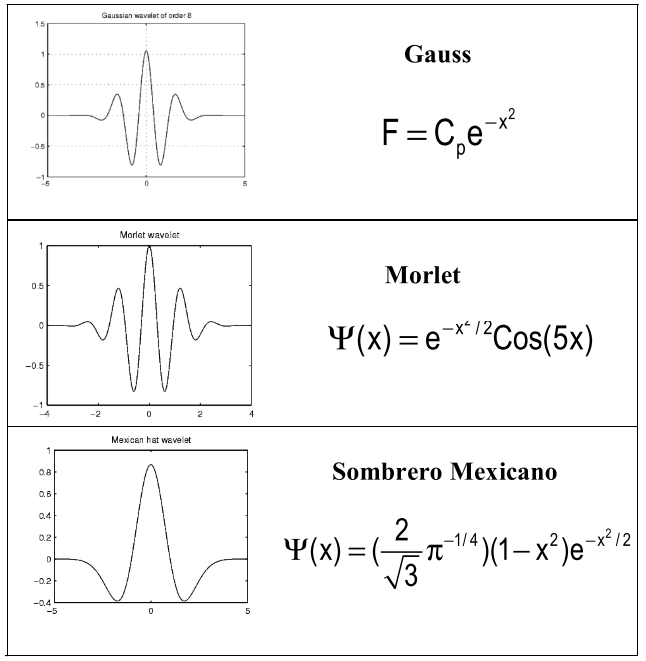
\includegraphics[scale=0.5]{Fig/7}
    \caption{Tipos de Wavelet Madres más utilizadas. Fuente:}
    \label{WM}
\end{figure}
Finalmente, la transformada de wavelet continua (CWT) se define como la correlación entre la señal a transformar $f(t)$ y la expresión de la familia de wavelets $\psi(a,b)(t)$:
\begin{equation}
    CWT f(u,s)= \int_{-\infty}^{\infty} f(t) \frac{1}{\sqrt{a}} \psi(\frac{t-b}{a})dt
\end{equation}

\subsection*{Transformada Wavelet Discreta}
Debido a la variabilidad de los parámetros de escala y traslación, en el marco continuo, es necesario discretizar el análisis con la finalidad 
de luego implementar un análisis computacional, ya que estos coeficientes generan una gran cantidad de datos. Para lograr esto, aproximamos las integrales con sumatorias y representamos la 
señal a estudiar como:
\begin{equation}
    \label{DWT}
 f(t) = \sum_{k}\sum_{j} c_{j,k}\phi (t) + \sum_{k}\sum_{j} d_{j,k}\psi (t)
\end{equation}
En la ecuación \ref{DWT} la señal $f(t)$ se aproxima como una sumatoria de funciones wavelet $\psi (t)$ y funciones de escala $\phi (t)$. Donde las funciones wavelet representan los detalles finos de la señal y las funciones escala 
realizan una aproximación. Con el fin de discretizar la función wavelet (ecuación \ref{WM}) se utiliza un muestreo exponencial para garantizar una mejor aproximación:
\begin{equation}
    \begin{split}
        &a=a_0^{-j}\\
        &b=nka_0^{-j}
    \end{split}
\end{equation}
Reemplazando los coeficientes de escalamiento y desplazamiento ahora discretizados en la ecuacion \ref{WM}:
\begin{equation}
    \psi_{j,k}(t) = a_0^{j/2} \psi (a_0^jt-kn)
\end{equation}
Si se desea obtener una aproximación en niveles de resolución muy finos es necesario que el factor de escala sea $a=2^{-j}$ y $n=1$ (Teorema de sampleo de Shannon's) lo que garantiza una resolución de 
$2^j$ (Debido a esto la señal resultante $f[n]$ tendra una longitud de $2^n$). Este procedemiento da como resultado:
\begin{equation}
    \psi_{j,k}(t) = 2^{j/2} \psi (2^jt-kn)
\end{equation}
De igual forma para las señales de escala se obtiene:
\begin{equation}
    \phi_{j,k}(t) = 2^{j/2} \phi (2^jt-kn)
\end{equation}
Una vez definida estas funciones podemos reescribir la ecuación \ref{DWT} como:
\begin{equation}
    f(t) = \sum_{k}\sum_{j} c_{j,k}2^{j/2} \phi (2^jt-kn)  + \sum_{k}\sum_{j} d_{j,k}2^{j/2} \psi (2^jt-kn)
\end{equation}

\end{document}